\documentclass{article}
%\usepackage{showkeys}
\usepackage{amsmath, amsfonts}
\usepackage{amsthm}
\usepackage{graphicx}
\usepackage{cite}
\usepackage{enumerate}
\usepackage{subfig}
\usepackage{textcomp}
\usepackage[margin=1in]{geometry}

\begin{document}
\begin{center}
\Large
Wigner Model Spike Detection Statistical Power Bounds \\
\normalsize
~\\
Michael Rawson\\
~\\
Advisor: Prof. Afonso Bandiera
\end{center}

\begin{abstract}

Perry et. al. \cite{perry} show that there is no statistical test for the spiked Gaussian Wigner model that solves the detection problem below the threshold $\lambda = 1$ with error approaching 0. The value of the second moment can give detection lower bounds on false positive errors (type I) and false negative errors (type II) for $\lambda < 1$. Using the trace, we calculate upper bounds for type I and type II errors while detecting spikes via hypothesis testing as $n \rightarrow \infty$.  Using Monte Carlo methods, we calculate upper bounds using statistical tests on the largest eigenvalues as $n \rightarrow \infty$.

\end{abstract}

\subsection*{Introduction}

Many data science problems involve detecting and recovering structure from noisy data. In random matrix theory, we seek to detect and recover a rank 1 square matrix added to a scaled, symmetric matrix with random entries. This model is called a spiked Wigner matrix.\\
\\
Spiked Wigner Matrix: 
$$Y = \lambda x x^T + \frac{1}{\sqrt{n}} W$$
For $x \in \mathbb{R}^n$ and $\|x\|_2^2 \rightarrow 1$ as $n \rightarrow \infty$ with entries drawn i.i.d. and $W \in \mathbb{R}^{n \times n}$ where $W$ symmetric and entries drawn i.i.d.\\
\\
The classical solution to this problem is principle component analysis (PCA). PCA analyzes the eigenvalues and eigenvectors of the matrix. In the 1950's, Wigner \cite{wigner} was looking into the distribution of the eigenvalues of symmetric random matrices. As $n \rightarrow \infty$, Wigner observed a distribution.\\
\\
Wigner Semicircle Distribution:
$$ f(x) = \frac{2}{\pi R^2}\sqrt{R^2-x^2} $$
For $-R \le x \le R$ and $f(x) = 0$ otherwise.\\
\\
Baik, Ben Arous, and P\'{e}ch\'{e} \cite{arous} showed that this distribution is very useful for detecting low rank matrices in the noise. It is shown that the top eigenvalue leaves the distribution when a strong signal (large $ \lambda $) is used. Here the threshold is $\lambda=1$. So when $\lambda>1$, the first principle component from PCA will detect or fail to detect a spike in the matrix as $n \rightarrow \infty$. \\
\\
Perry, Wein, Bandiera, and Moitra \cite{perry} show a lower bound on the statistical error, based on the second moment, when $\lambda$ is below the threshold. Two types of error need to be considered, the error of detecting a spike when a spike does not exist ($\lambda=0$) called Type I error and the error of detecting no spike when a spike does exist ($\lambda>0$) called Type II error. Intuitively, for $\lambda$ close to $0$, we would expect the structure to be lost to the relatively large noise and low error unattainable. Perry et. al. show this in \cite{perry} Figure 1.\\
\\
Now that we have tight lower bounds (depending on the sampled distribution), we examine upper bounds with statistical hypothesis testing. Specifically, hypothesis testing calculates the probability of observing a sample given a hypothesis. The statistical power of a binary hypothesis test is the probability of rejecting a hypothesis given the hypothesis is false.\\
\\
Statistical Power:
$$ \texttt{Power} = P(\texttt{reject } H_0|H_0 \texttt{ is false}) $$

In order to analyze the statistical power, we can write down and integrate the distribution of some function $f$ of $Y$, $f(Y)$, where the distribution that x and W are sampled from is know. But, for some functions $f$ the distribution of $f(Y)$ is very complicated so we approximate the distribution with the Monte Carlo method. The simplest Monte Carlo method approximates the mean of a distribution by calculating the empirical mean of a large number of i.i.d. samples which follows from the weak Law of Large Numbers.\\
\\
Weak Law of Large Numbers:
$$\overline X_n \rightarrow \mu \texttt{ in probability as } n \rightarrow \infty $$
For $\overline X_n$ the empirical mean of n samples.\\
\\
Proof:\\
Assume $\texttt{Var}(X_i) = \sigma^2$ for all $i$. Then
$$\texttt{Var}(\overline X_n) = \texttt{Var}(\frac 1n (X_1+...+X_n)) = \frac 1n^2 \texttt{Var}(X_1+...+X_2) = \frac{n \sigma^2}{n^2} = \frac{\sigma^2}{n} $$
$$\mathbb{E}(\overline X_n)=\mu$$
By Chebyshev's inequality,
$$P(|\overline X_n-\mu|\ge \epsilon) \le \frac{\sigma^2}{n \epsilon^2}$$
Implies,
$$P(|\overline X_n-\mu | < \epsilon) \ge 1-\frac{\sigma^2}{n \epsilon^2}$$
Then,
$$\lim_{n \rightarrow \infty} P(|\overline X_n-\mu| < \epsilon) = 1 \qed $$
\\
\\
The next approximation from the Monte Carlo method that we use is the approximation of the variance.\\
\\
Theorem:
$$\frac 1n \sum_{i=1}^n (X_i - \overline X_n)^2 \rightarrow \sigma^2 \texttt{ in probability as } n \rightarrow \infty $$
For $\overline X_n$ the empirical mean of n samples.\\
\\
Proof:\\
$$ \frac 1n \sum_{i=1}^n (X_i - \overline X_n)^2 
     = \frac 1n \sum_{i=1}^n X_i^2 - 2 \overline X_n \frac 1n \sum_{i=1}^n (X_i) + \overline X_n^2$$
$$ \rightarrow \sigma^2 + \mu^2 - \mu^2 \texttt{ in probability as } n \rightarrow \infty $$

Since $ \overline X_n \rightarrow \mu $ and $ \frac 1n \sum_{i=1}^n X_i^2 \rightarrow \sigma^2 + \mu^2 $ by Law of Large Numbers \qed

Now, with the approximate mean and variance, we can approximate distributions and measure statistical power and error.

\subsection*{Monte Carlo Simulation}

We let x and W be drawn from normal distributions. Then Trace(Y) is a random variable that is normally distributed since the sum of normal random variables is a normal random variable. The Monte Carlo simulation gives us the mean and variance of Trace(Y) so we infer the distribution of Trace(Y).\\
\\
For the weak signal $\lambda = 0.5$, we plot the lower bound from Perry et. al. \cite{perry} and the upper bound from Trace(Y) for large n in Fig. \ref{fig:plot_traceY_lambda_50}. For $\lambda = 0.5$, the upper and lower bounds are relatively close. However, for the strong signal $\lambda = .99$, we plot the lower bound from Perry et. al. \cite{perry} and the upper bound from Trace(Y) for large n in Fig. \ref{fig:plot_traceY_lambda_99} and the gap is much larger.

\begin{figure}
    \centering
    {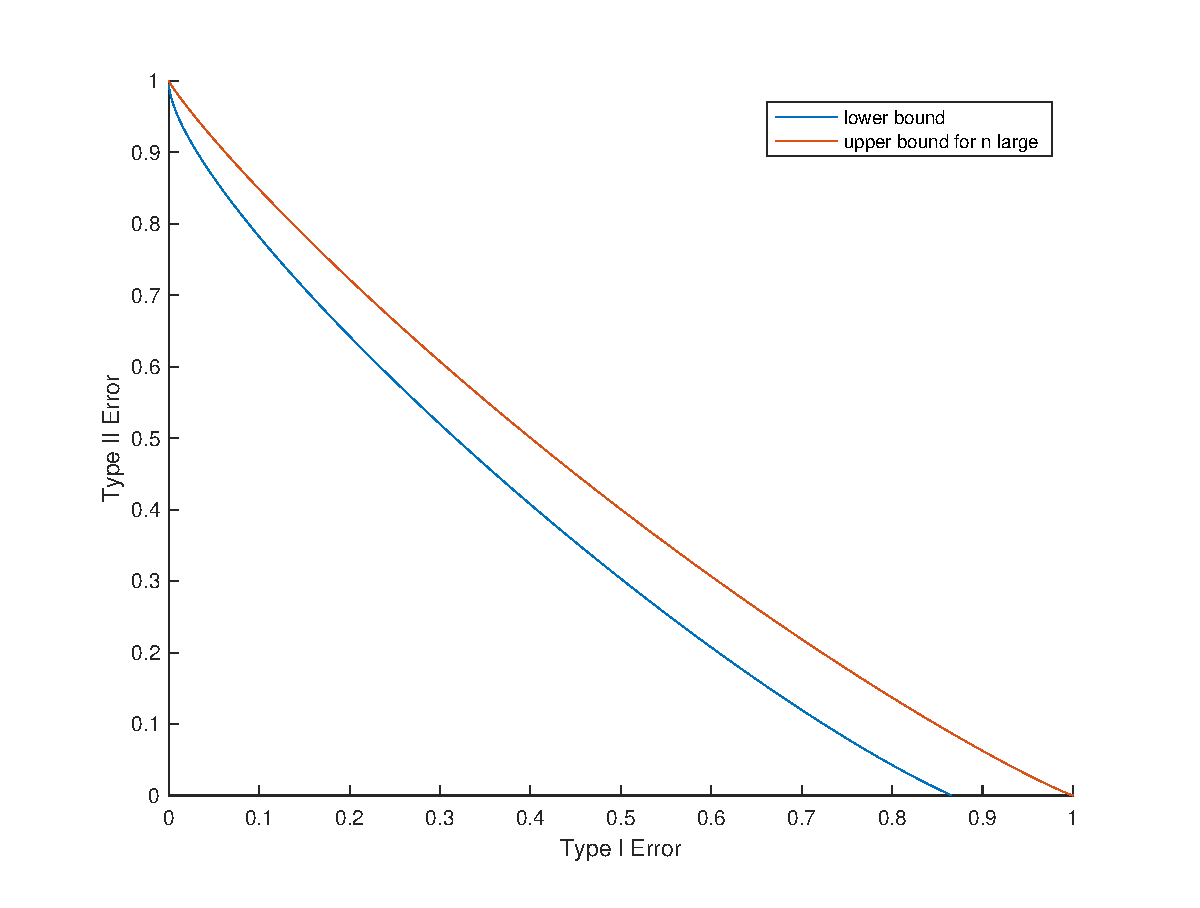
\includegraphics[width=11cm]{plot_traceY_lambda_50.eps} }
    \caption{ Plot error bound from Trace(Y) where $\lambda = 0.5$}
	\label{fig:plot_traceY_lambda_50}
\end{figure}

\begin{figure}
    \centering
    {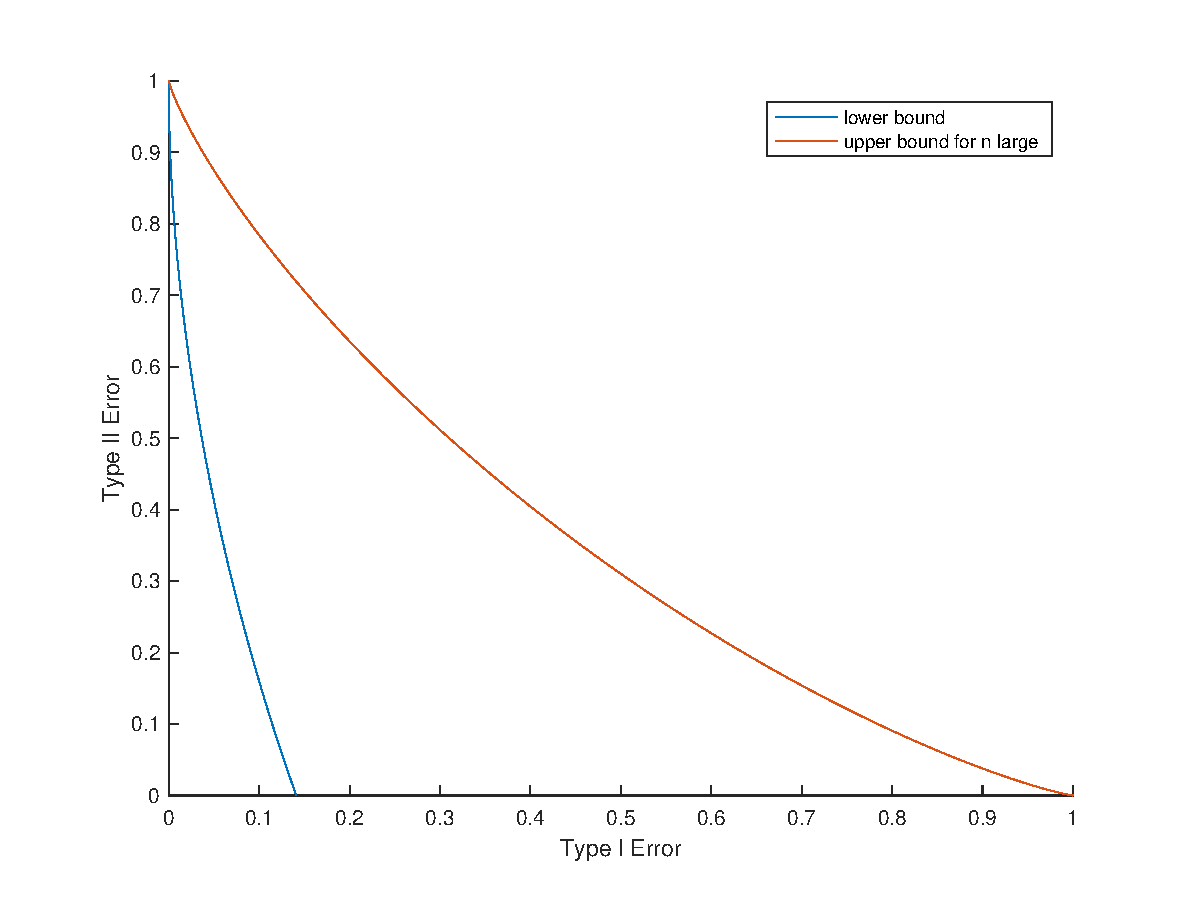
\includegraphics[width=11cm]{plot_traceY_lambda_99.eps} }
    \caption{ Plot error bound from Trace(Y) where $\lambda = 0.99$}
	\label{fig:plot_traceY_lambda_99}
\end{figure}

Seeking a lower upper bound, we consider the largest eigenvalue of Y. We know the eigenvalues of Y have a Wigner semicircle distribution in the limit. However, the top eigenvalue has a Tracy-Wisdom distribution, which can be accurately approximated by a gamma distribution, shown by Marco Chiani (2012) \cite{chiani} . We parametrize a gamma distribution with the Monte Carlo simulation. For $\lambda = 0.5$, We plot the lower bound from Perry et. al. \cite{perry} and the upper bound from the largest eigenvalue of Y along with the upper bound from Trace(Y) for large n in Fig. \ref{fig:plot_top_eigY_lambda_99}. We notice this upper bound is much lower than that the Trace(Y) yields. Yet, for $\lambda = 0.99$, the performance does not continue to out perform.


\begin{figure}
    \centering
    {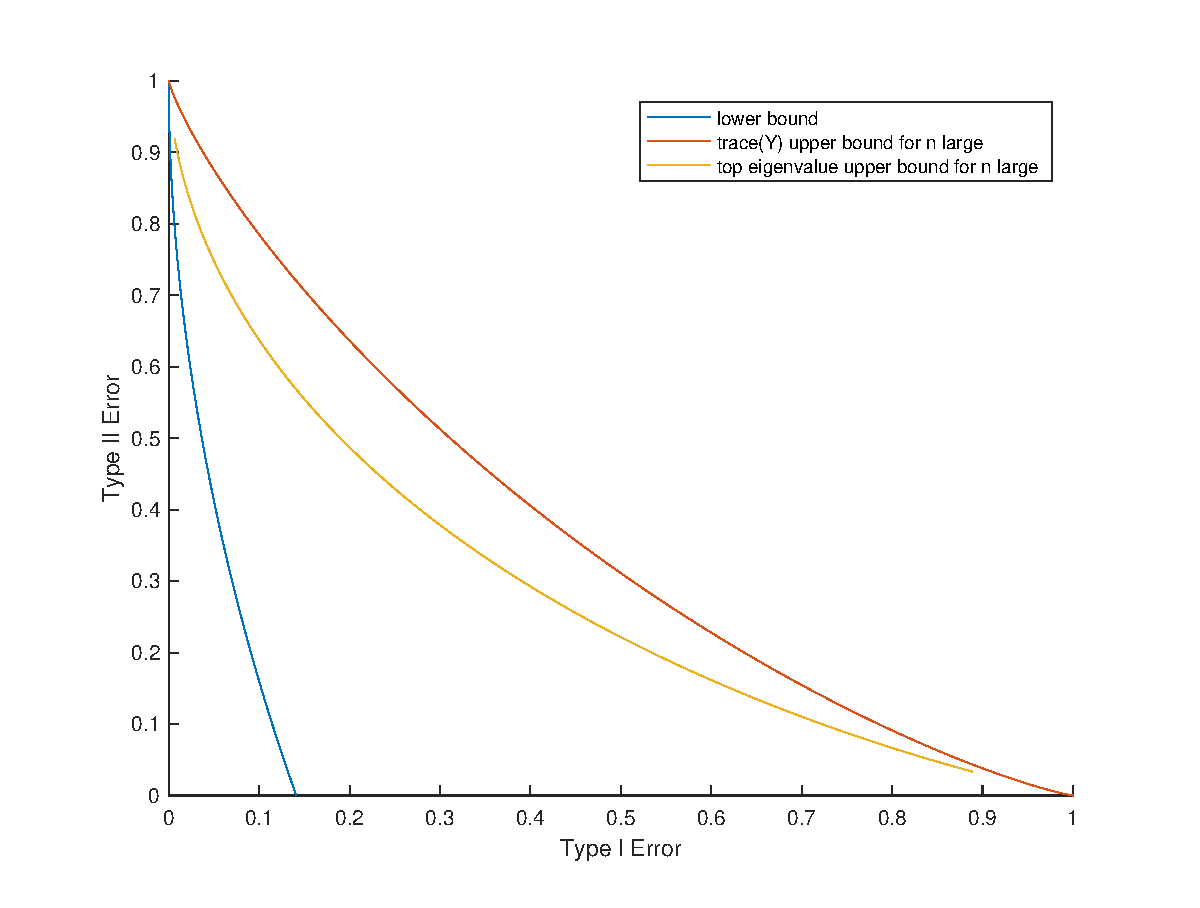
\includegraphics[width=11cm]{plot_top_eigY_lambda_99.eps} }
    \caption{ Plot error bound compare Trace(Y) and top eigenvalue of Y where $\lambda = 0.99$}
	\label{fig:plot_top_eigY_lambda_99}
\end{figure}

\begin{figure}
    \centering
    {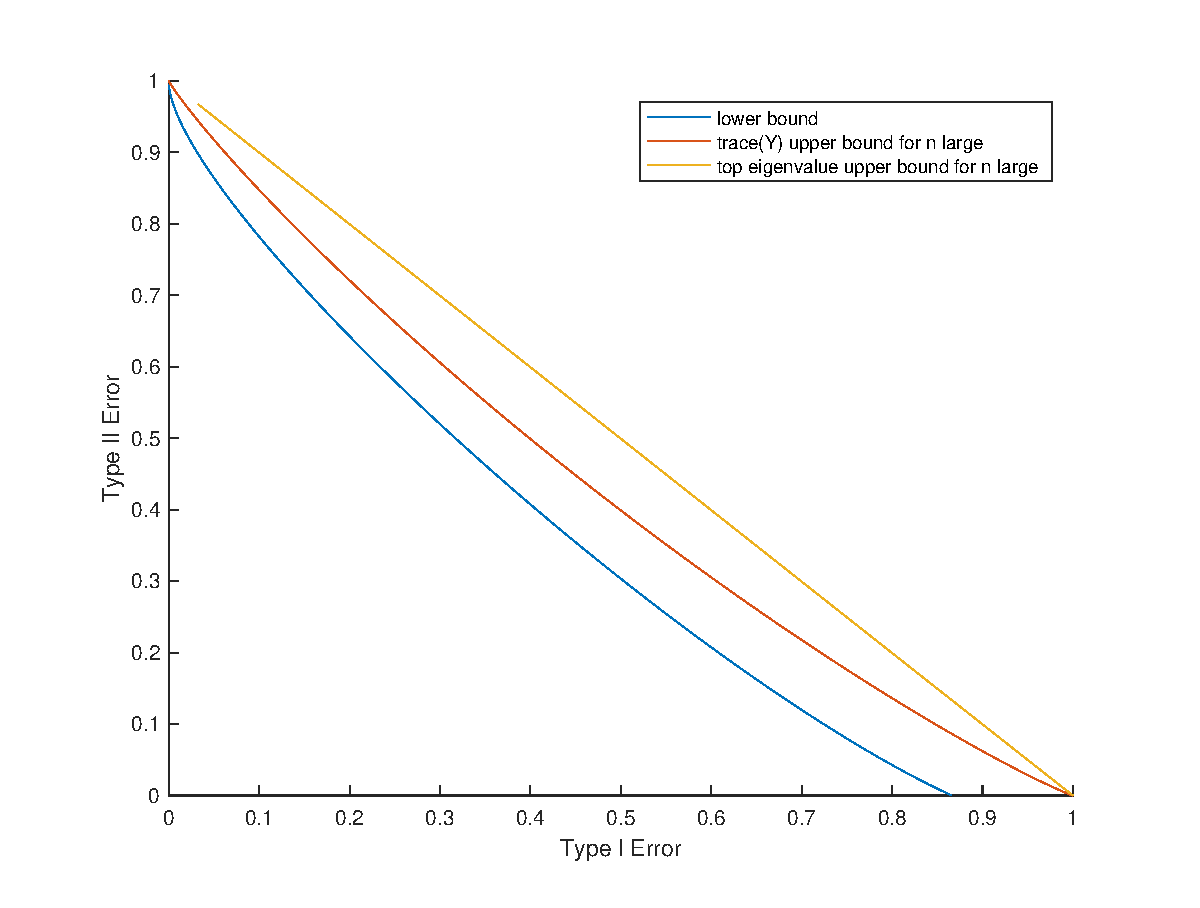
\includegraphics[width=11cm]{plot_top_eigY_lambda_50.eps} }
    \caption{ Plot error bound compare Trace(Y) and top eigenvalue of Y where $\lambda = 0.5$}
	\label{fig:plot_top_eigY_lambda_50}
\end{figure}


\subsection*{Analysis}
We mathematically analyze the trace of a spiked Wigner matrix for spike detection.\\
\\
Spiked Gaussian Wigner Matrix: 
$$Y = \lambda x x^T + \frac{1}{\sqrt{n}} W$$
$$W_{i,j} \sim N(0,1) \quad \forall i>j$$
$$W_{i,i} \sim N(0,2) \quad \forall i$$
For $W \in \mathbb{R}^{n \times n}$ where $W$ symmetric and entries drawn i.i.d. and $x \in \mathbb{R}^n$\\
When $n = \infty$ let $x_i = \frac{1}{\sqrt{n}}$ then $\|x\|_2^2 = 1$\\
\\
Let the null hypothesis ($H_0$): $\lambda = 0$
$$ \mathbb{E} \texttt{ Trace}(W)/\sqrt{n} =  \frac {1}{\sqrt{n}} \sum_i \mathbb{E} W_{i,i} = 0$$
$$ Var \texttt{ Trace}(W)/\sqrt{n} =  \frac {1}{n} \sum_i Var (W_{i,i}) = 2$$

$$ \texttt{ Trace}(W)/\sqrt{n} \sim N(0,2) $$
\\
Let the alternative hypothesis ($H_1$): $\lambda > 0$
$$ \mathbb{E} \texttt{ Trace}(\lambda x x^T + W/\sqrt{n})$$
$$= \texttt{ Trace}(\lambda x x^T) + \mathbb{E}\texttt{ Trace}(W/\sqrt{n})$$
$$= \lambda \sum_i \frac 1n + 0$$
$$= \lambda $$

$$ Var \texttt{ Trace}(\lambda x x^T + W/\sqrt{n}) $$
$$ = \frac {1}{n} \sum_i Var (W_{i,i}) = 2$$

$$ Var(Y) \sim N(\lambda,2) $$

Now, with this analysis in hand we plot the statistical upper bounds and we verify that our Monte Carlo simulation from earlier gave approximately the correct bound for $\lambda = 0.99, 0.5$, see Fig. \ref{fig:plot_traceY_lambda_99_analytic} and Fig. \ref{fig:plot_traceY_lambda_50_analytic}

\begin{figure}
    \centering
    {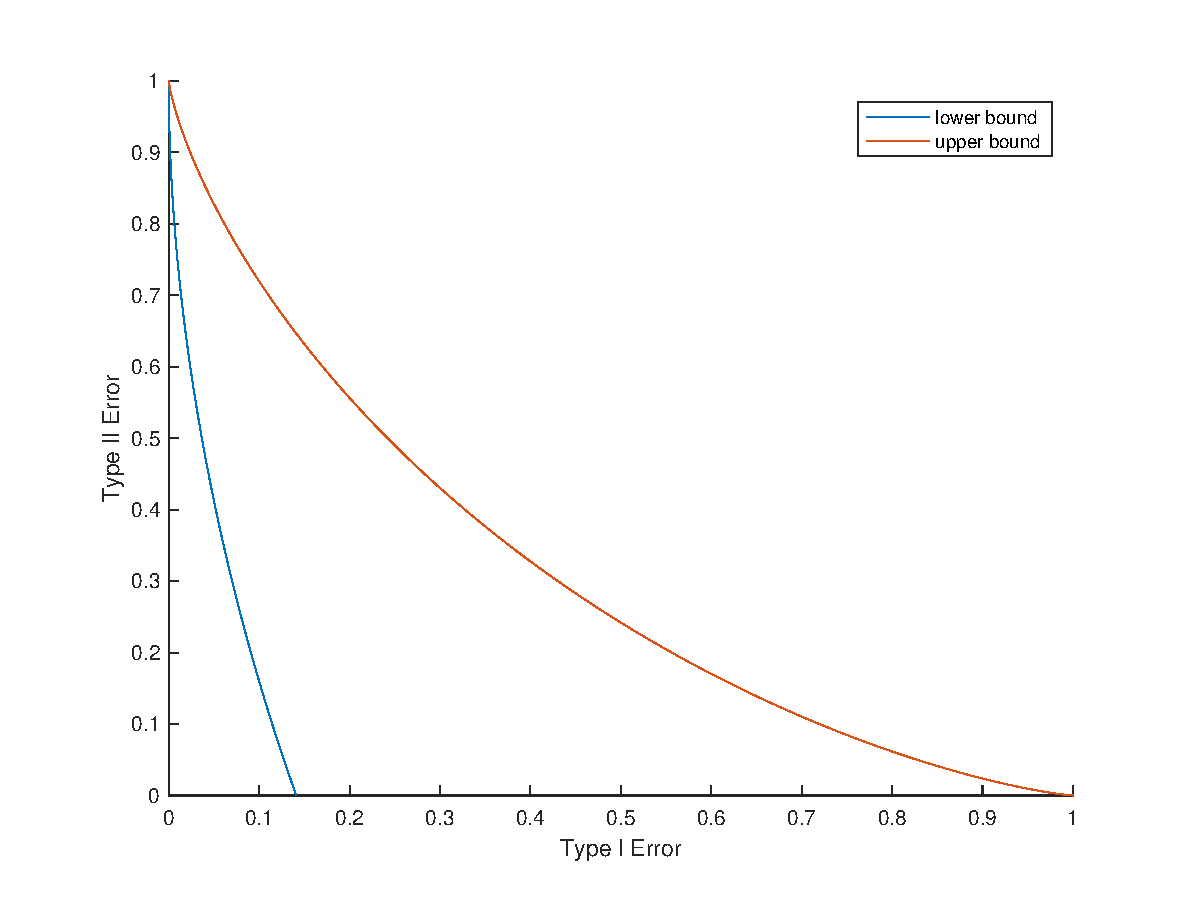
\includegraphics[width=11cm]{plot_traceY_lambda_99_analytic.eps} }
    \caption{ Plot error bound analysis Trace(Y) where $\lambda = 0.99$}
	\label{fig:plot_traceY_lambda_99_analytic}
\end{figure}

\begin{figure}
    \centering
    {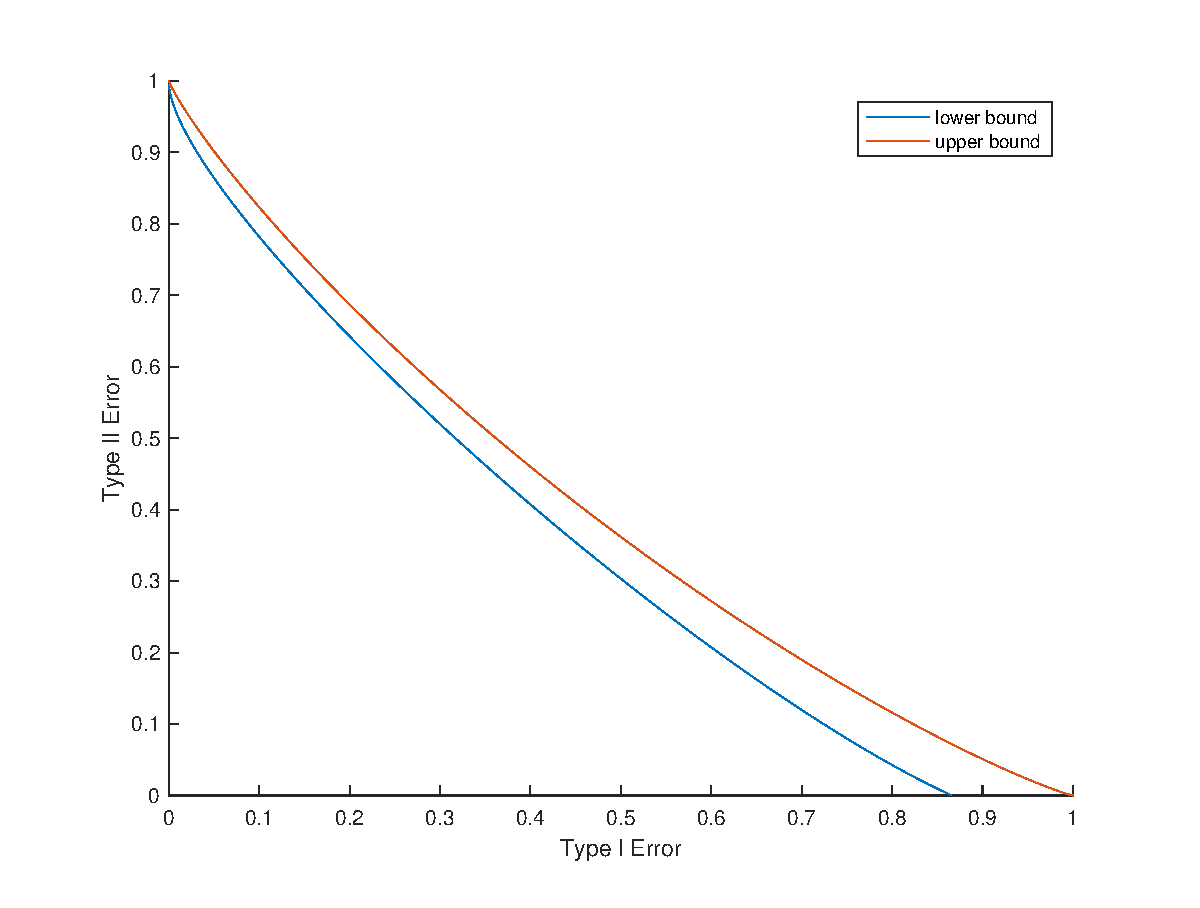
\includegraphics[width=11cm]{plot_traceY_lambda_50_analytic.eps} }
    \caption{ Plot error bound analysis Trace(Y) where $\lambda = 0.5$}
	\label{fig:plot_traceY_lambda_50_analytic}
\end{figure}

\subsection*{Conclusion}
We have shown that Monte Carlo simulations can be effective for identifying statistical bounds. We created upper bounds for the spike detection in a Wigner model matrix and found an example where two bounds switch in terms of performance with respect to $\lambda$. Future work includes finding better bounds and generalizing the bounds. This work is for Gaussian distributions, but future work could generalize this to non-Gaussian distributions or neighboring models such as the Wishart model.

\bibliographystyle{plain}

\bibliography{Project_PCA.bib}

\end{document}







